\section{Motivation and Scope}
\label{motivacao}

The use of \gls{ML} models in the educational domain, called \gls{EDM} has gained considerable attention in recent literature \cite{Romero2020EducationalSurvey}. The \gls{EDM} encompasses a diverse array of applications, ranging from predicting student dropout rates \cite{Araque2009FactorsRates, Aguiar2015WhoWhy} to facilitating the creation of personalized learning paths \cite{Fancsali2018IntelligentOffs}. Beyond predictive accuracy, the interpretability of these models can be critical for their responsible integration into educational settings.

In certain contexts, the accuracy of predictions may even take a back seat to the insights gained from model explanations. For instance, in the field of educational assessment, \gls{EDM} has emerged as a potent tool for analyzing \gls{LSA} datasets. These datasets are invaluable for identifying key variables impacting educational systems, aiming to provide empirical evidence to inform discussions on educational policies  \cite{Hernandez-Torrano2021ModernLiteratureb}. \gls{EDM} allows for the extraction of knowledge from significant relationships within these extensive databases \cite{Gamazo2020AnTechniques}. Unlike traditional approaches that rely on theoretical distribution, \gls{EDM} models are developed and validated using empirical data. This flexibility enables researchers to revisit and refine existing theoretical models \cite{Huang2003InstitutePolicymakers}.

There are many discussions of what has consisted of a model explanation, and they can be delivered in many ways \cite{Guidotti2018AModels}. Feature-based explanations are among the most prevalent, focusing on identifying critical features that influence model output at either the example level (local) or the sample level (global). At the global level, these feature-based explanations are commonly conveyed through summary metrics reporting scores of the overall feature contribution or through plots detailing its different effects over the data sample \cite{SilvaFilho2023AAchievement}.

Moreover, the explanation methods can be internal to the model (intrinsically) as the coefficients of linear regression and the path of a tree or by applying a second model that analyzes the initial one (post-hoc). Another criterion to classify these methods is related to their generalizability, whether they are model-specific or model-agnostic. While every intrinsic method is specific, all model-agnostic work is in a post-hoc framework \cite{SilvaFilho2021InterpretingEffects}.

This thesis is principally concerned with the critical evaluation of the global explanations in the post-hoc framework, which has raised concerns due to two key challenges. The first challenge pertains to the predictive model itself: high predictive performance is not a sufficient indicator that the model has captured the true relationships in the data. Rather, it may be exploiting spurious correlations, thereby limiting the validity of any insights extracted from the model \cite{Mittelstadt2019ExplainingAI}. The second challenge, which is the focus of this thesis, lies in the explanation methods. Even if the model could accurately captures the true data relationships, the explanation methods may not effectively illustrate how the model actually works \cite{Rudin2019StopInstead, Mittelstadt2019ExplainingAI}.

Incorporating domain knowledge and ensuring the model's structural integrity can help mitigate the first issue \cite{Frye2021ShapleyManifold, Zhao2021CausalModels}. However, the problem of collinearity - where variables are interdependent - remains a significant issue for the second challenge \cite{Hooker2019UnrestrictedImportance}. Collinearity becomes problematic when overlooked in the explanations. This issue is especially pronounced in methods that rely heavily on the structure of the model while neglecting the crucial interrelationships within the datasets.

Recently, in the \gls{EDM} field, many scholars have been relying on global explanations derived from \gls{XAI}  techniques that assume data independence in an attempt to extract knowledge from data. However, data independence might be a strong assumption for many \gls{EDM} tasks, especially when using structural data based on personal and contextual information. This kind of data tends to be highly correlated with strong inter-feature dependencies. For example, in predicting student success based on \gls{LSA} data, socioeconomic variables often have a significant influence on student achievement, along with other contextual variables such as demographics, school environment and process, parental education level, and access to educational resources \cite{coleman1968equality, Andrade2008OBrasileira}. 

Standard supervised \gls{ML} is widely recognized for its emphasis on performance. This focus can lead to learned functions that do not accurately reflect the true data-generating process behind student success (first challenge). Consequently, insights into this phenomenon are valuable only when the predictive function is thoroughly explained within the context of the data distribution used for training. An explainable approach that overlooks the data interrelationships may not yield reliable explanations (the second challenge).  This issue becomes more critical when data dependencies naturally introduce biases in the explanations. For example, low relevant variables can be attributed a high relevance only due to co-dependency with a high relevant variable. 

A common strategy of global post-hoc techniques involves modifying the value of a specific feature as a sign of its impact on the model \cite{Scholbeck2020SamplingInterpretations}. Essentially, features are manipulated to generate new predictions. From a model-centric viewpoint, ignoring data relationships in these interventions can lead to misalignment with the actual data distribution. This may lead to the creation of unrealistic data points and, consequently, the potential for unusual predictions. For example, Figure \ref{fig:extrapolation_introduction} illustrates this situation in a dataset that controls the weight and height of adults.  If data dependencies are overlooked during interventions, scenarios like very low weight paired with very tall height might be erroneously generated (red points in the Figure), which are improbable or even physically implausible in reality. Predictions based on these unlikely data points can thus yield unreliable results, significantly reducing the practical value of the model's explanations. This issue is referred to as the "extrapolation" problem \cite{Molnar2022GeneralModels, Rudin2019StopInstead}. This can also pose a problem in educational datasets, where points outside the distribution are used to compute feature effects and inform decision-making. 

\begin{figure}[ht!]
\centering
  \fcolorbox{gray}{white}{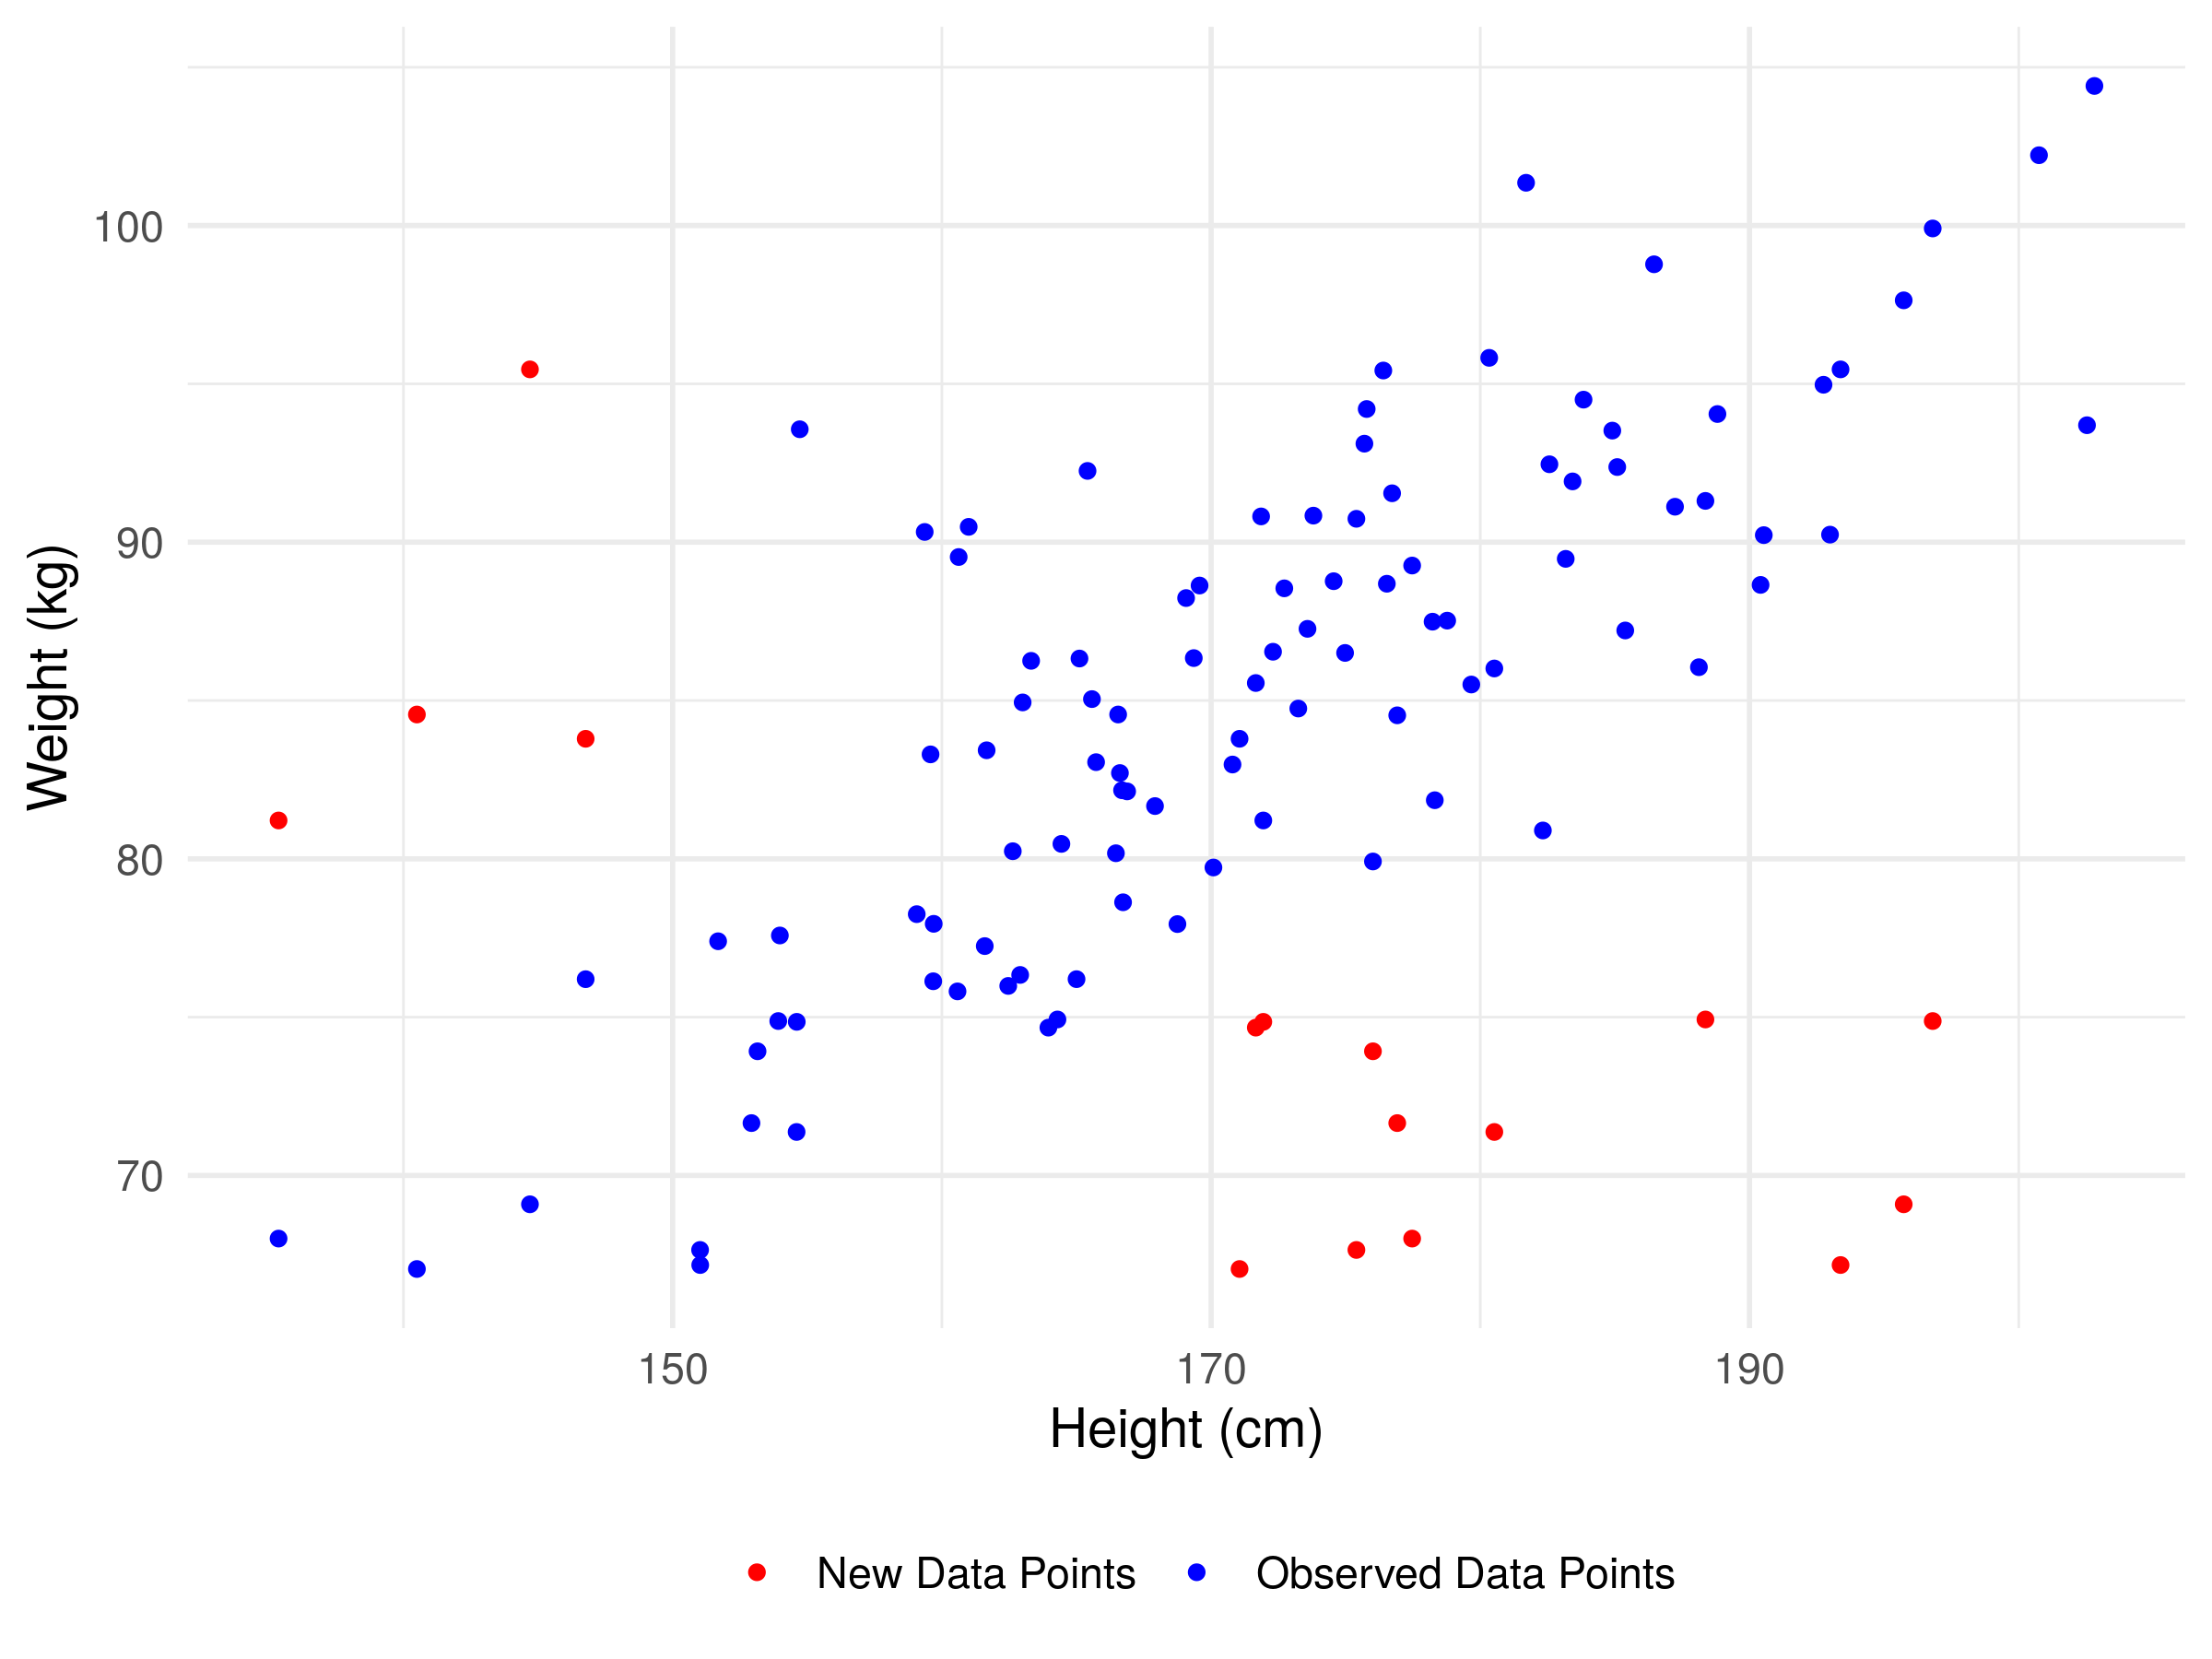
\includegraphics[width=0.7\textwidth]{images/captitulo1/extrapolation_introduction.png}}
  \caption{Illustration of the extrapolation problem. Blue dots are the observed data points. Red dots are new data points derived from interventions that do not align with the actual data distribution.}
    \label{fig:extrapolation_introduction}
\end{figure}

 
In light of these challenges, this thesis is motivated by the need for more rigorous methods to determine global feature contributions in \gls{EDM}, especially when feature independence cannot be assumed. This work is significant not only for educational practitioners engaged in data-driven tasks, who would benefit from more reliable interpretations of \gls{ML} models, but also for the ML research community. Researchers can generalize the methods and ideas presented here to advance the literature on \gls{XAI}, fostering a more comprehensive adoption of ML systems.
